\texttt{MINIMAX}
\begin{figure}[h]
    \centering
    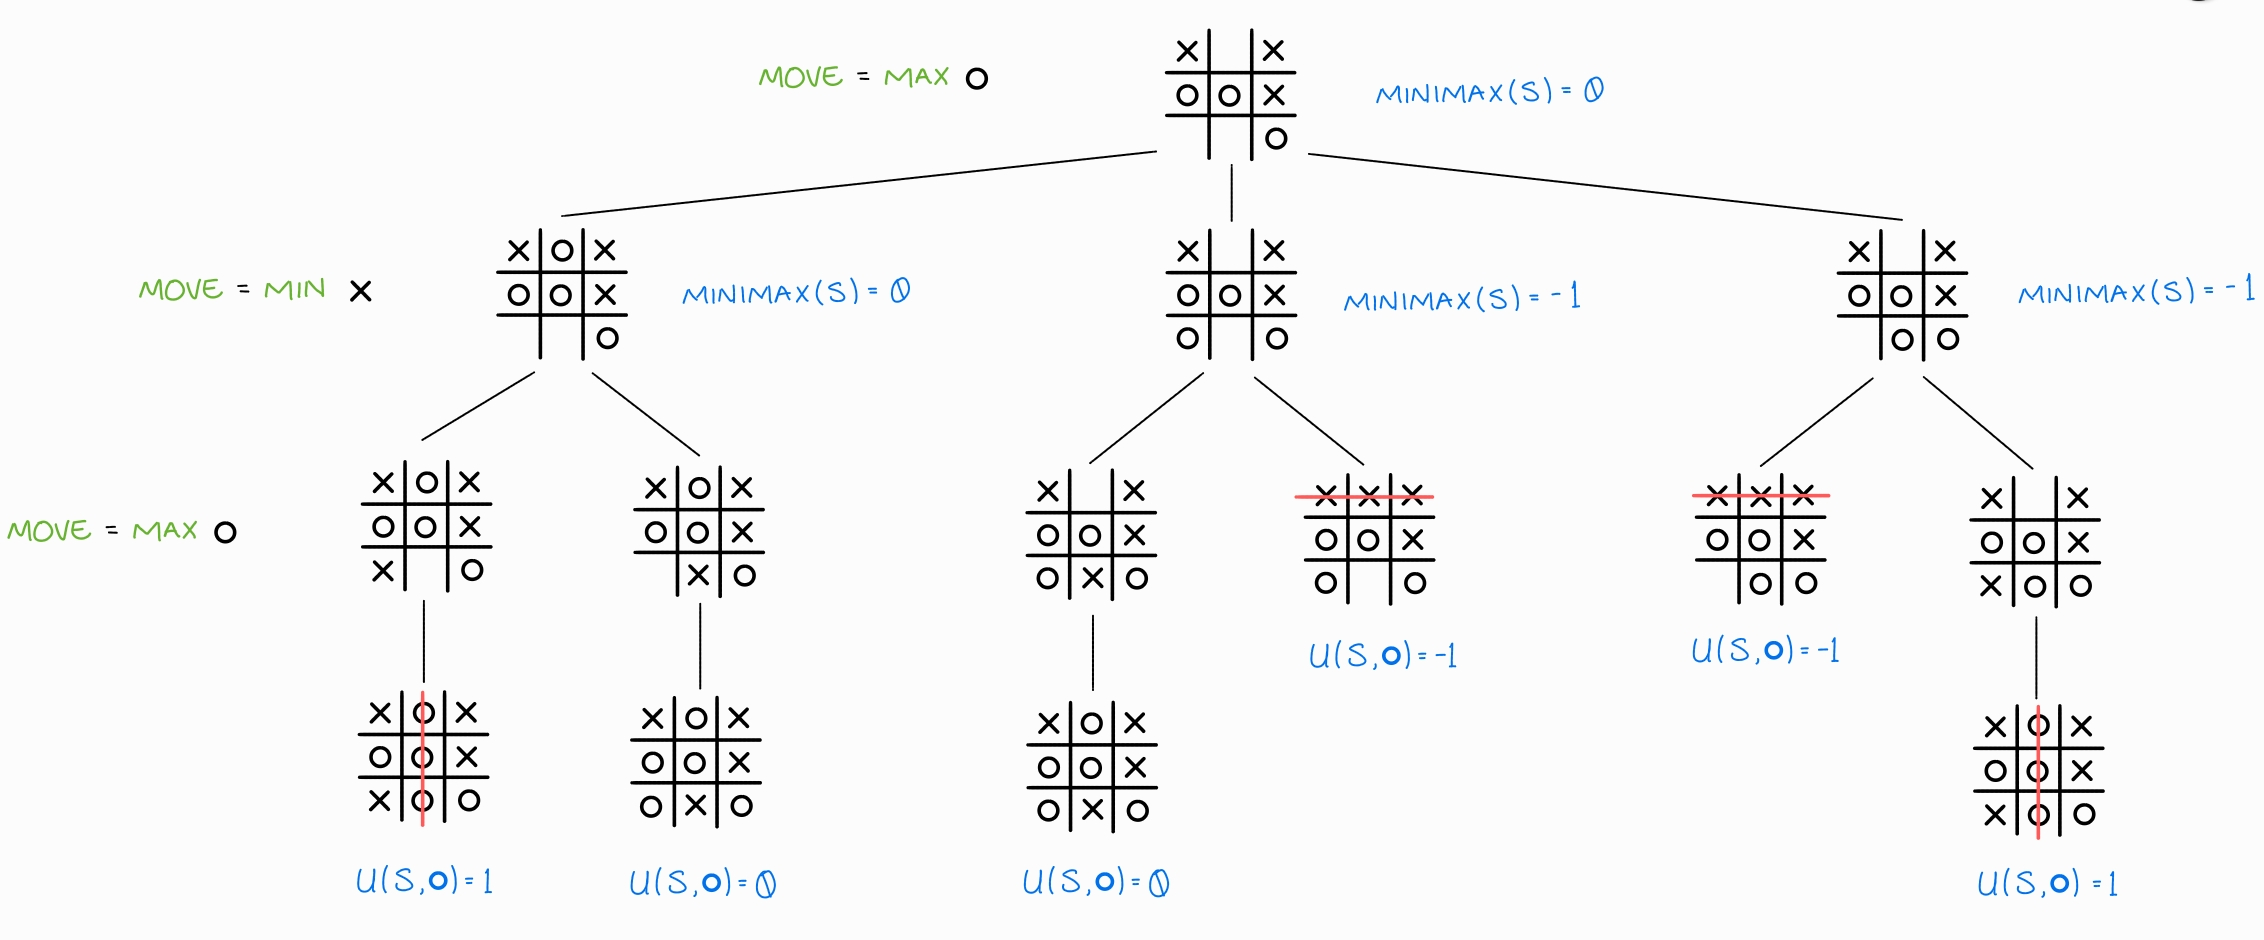
\includegraphics[width=1\textwidth]{fe11.jpg}
\end{figure}

Recordemos que:
\[
\operatorname{Minimax}(s)=
\begin{cases}
U(s,\mathrm{MAX}) & \text{si } s \in F,\\[4pt]
\max_{a}\operatorname{Minimax}(T(s,a)) & \text{si } \mathrm{Move}=\mathrm{MAX},\\[4pt]
\min_{a}\operatorname{Minimax}(T(s,a)) & \text{si } \mathrm{Move}=\mathrm{MIN}.
\end{cases}
\]

Como la raíz es MAX:

\[
\text{MINIMAX}(s_0) = \max(\text{MINIMAX}(s_1), \text{MINIMAX}(s_2), \text{MINIMAX}(s_3)).
\]

\begin{itemize}
    \item \(\text{MINIMAX}(s_1) = \min(+1, 0) = 0\)
    \item \(\text{MINIMAX}(s_2) = \min(-1, 0) = -1\)
    \item \(\text{MINIMAX}(s_3) = \min(-1, +1) = -1\)
\end{itemize}

\[
\therefore \text{MINIMAX}(s_0) = \max(0, -1, -1) = 0
\]


